\documentclass[12pt,letterpaper]{article}
\usepackage[utf8]{inputenc}
\usepackage[spanish]{babel}
\usepackage{graphicx}
\usepackage[left=2cm,right=2cm,top=2cm,bottom=2cm]{geometry}
\usepackage{graphicx} % figuras
% \usepackage{subfigure} % subfiguras
\usepackage{float} % para usar [H]
\usepackage{amsmath}
%\usepackage{txfonts}
\usepackage{stackrel} 
\usepackage{multirow}
\usepackage{enumerate} % enumerados
\renewcommand{\labelitemi}{$-$}
\renewcommand{\labelitemii}{$\cdot$}
% \author{}
% \title{Caratula}
\begin{document}

% Fancy Header and Footer
% \usepackage{fancyhdr}
% \pagestyle{fancy}
% \cfoot{}
% \rfoot{\thepage}
%

% \usepackage[hidelinks]{hyperref} % CREA HYPERVINCULOS EN INDICE

% \author{}
\title{Caratula}

\begin{titlepage}
\begin{center}
\large{UNIVERSIDAD PRIVADA-DE-TACNA}\\
\vspace*{-0.025in}
\begin{figure}[htb]
\begin{center}

\includegraphics[width=8cm]{./Imagenes/logo}
\end{center}
\end{figure}
\vspace*{0.15in}
INGENIERIA DE SISTEMAS  \\

\vspace*{0.5in}
\begin{large}
TITULO:\\
\end{large}

\vspace*{0.1in}
\begin{Large}
\textbf{INFORME DE LABORATORIO No 01}\\
\end{Large}

\vspace*{0.3in}
\begin{Large}
\textbf{CURSO:} \\
\end{Large}

\vspace*{0.1in}
\begin{large}
INTELIGENCIA DE NEGOCIOS\\
\end{large}

\vspace*{0.3in}
\begin{Large}
\textbf{DOCENTE(ING):} \\
\end{Large}

\vspace*{0.1in}
\begin{large}
 Patrick Cuadros Quiroga\\
\end{large}

\vspace*{0.2in}
\vspace*{0.1in}
\begin{large}
Estudiante: \\ 
Sharon Sosa Bedoya          (2016054460) \\
\end{large}
\end{center}

\end{titlepage}


\tableofcontents % INDICE
\thispagestyle{empty} % INDICE SIN NUMERO
\newpage
\setcounter{page}{1} % REINICIAR CONTADOR DE PAGINAS DESPUES DEL INDICE

\section{INFORMACIÓN GENERAL} 

\begin{itemize}
\subsection{Objetivos:}
	\item Conocer los fundamentos sobre como realizar una Gestion de Base de Datos con Oracle.
	\item Poder instalar correctamente una instancia.
\subsection{Equipos, materiales, programas y recursos utilizados:}
	\item Virtualización activada en el BIOS.
	\item Windows 10 64bit: Pro, Enterprise o Education, con al menos 4GB de RAM.
	\item Docker Desktop
	\item Oracle SQL Developer para Windows
	\item Microsoft SQL Server 2017 o superior

\end{itemize}

\section{PROCEDIMIENTO} 

\begin{itemize}
\subsection{Parte 1: Conectar a SQL Server desde Power BI Desktop }
	\item Para realizar los gráficos en PowerBi Desktop primero debemos conectarnos con nuestra base de datos, que ya tiene que tener la base de datos "AdventureWorks 2017".  \\Abrimos nuestro PowerBi desktop y procedemos a realizar la conexión a SQL server.
	\begin{figure}[h]
	\begin{center}
	\fbox{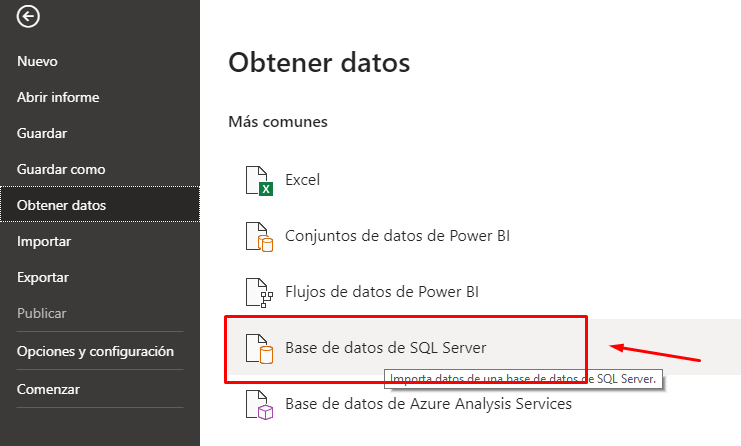
\includegraphics[width=12cm]{./Imagenes/tarea1}}
	\end{center}
	\end{figure}

\begin{figure}[h]
	\begin{center}
	\fbox{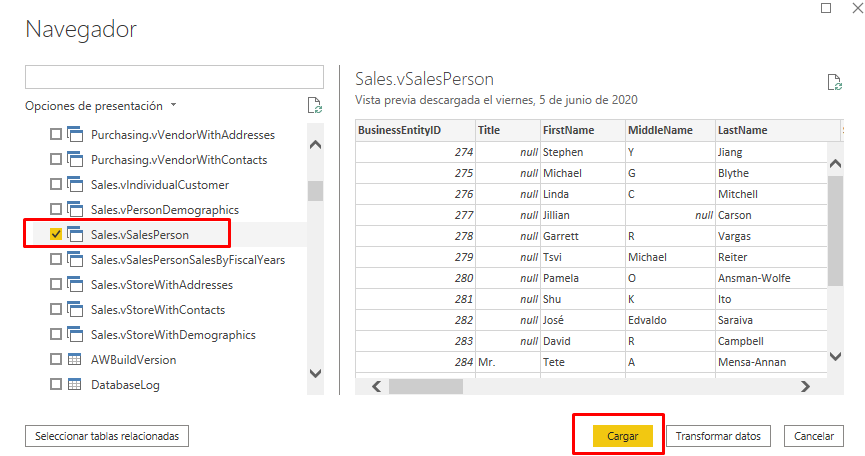
\includegraphics[width=13cm]{./Imagenes/tarea1_1}}
	\end{center}
	\end{figure}
\clearpage
	\begin{figure}[h]
	\begin{center}
	\fbox{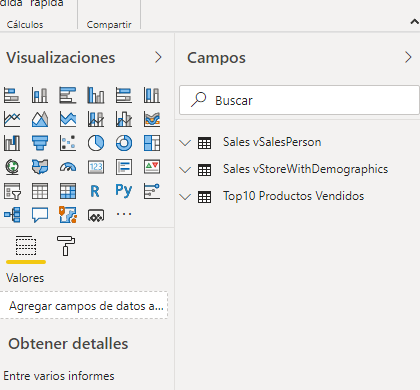
\includegraphics[width=11cm]{./Imagenes/tarea1_2}}
	\end{center}
	\end{figure}

	\item Una vez terminado de cargas los datos que necesitaremos, podremos visualizarlo en el panel lateral derecho de nombre "Campos".
	
     
\subsection{Parte 2: : Adicionar Gráficos al Reporte}
	\item En la parte 2 realizaremos los gráficos con la información de la base de datos que seleccionamos. Utilizaremos del panel de Visualizaciones los diferentes gráficos que nos ofrecen.

\begin{itemize}
	\item{\textbf{1. Cantidad de Ventas del personal: }} Gráfico de Columna Apilada que nos muestra el reporte de la cantidad de ventas de cada personal de ventas.
	\item {\textbf{2. Número de Empleados por especialidad: }}En el gráfico de Pie, muestra los la cantidad de empleados que tiene la empresa según su especialidad.
	\item {\textbf{3. Top 10 Productos vendidos: }}El gráfico de Donut, muestra el top 10 de los productos más vendidos. Podremos visualizarlo representados en los diferentes colores en el gráfico.
	\item {\textbf{4. Ventas Anuales y Beneficios Anuales: }}En el segundo gráfico de Columna Apilada podremos visualizar la cantidad de ventas anuales y los beneficios que ha traido. 
	\end{itemize}

\begin{figure}[h]
	\begin{center}
	\fbox{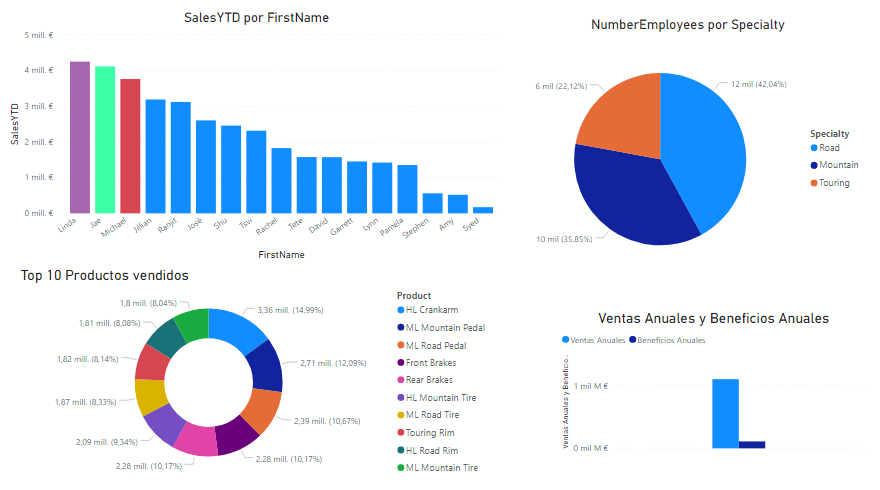
\includegraphics[width=15cm]{./Imagenes/tarea2}}
	\end{center}
	\end{figure}
		
\clearpage

\subsection{Parte 3: Publicar el reporte en el portal de Power BI}
	\item Cuando los gráficos esten listos, seleccionamos la opción de "Publicar" que nos ofrece PowerBi y poder subirlo a nuestra "Área de Trabajo". Cuando damos a "Aceptar" el archivo se irá subiendo a nuestra cuenta.

\begin{figure}[h]
	\begin{center}
	\fbox{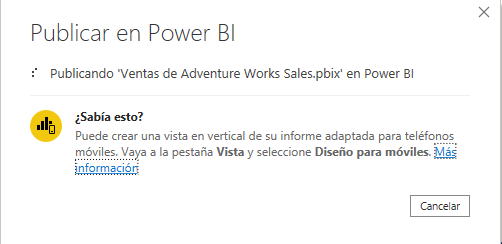
\includegraphics[width=11cm]{./Imagenes/tarea3}}
	\end{center}
	\end{figure}

\item Una vez se haya terminado de subir, abrimos nuestra cuenta desde la página web de Microsoft PowerBi y podremos visualizar nuestro trabajo ahí.

\begin{figure}[h]
	\begin{center}
	\fbox{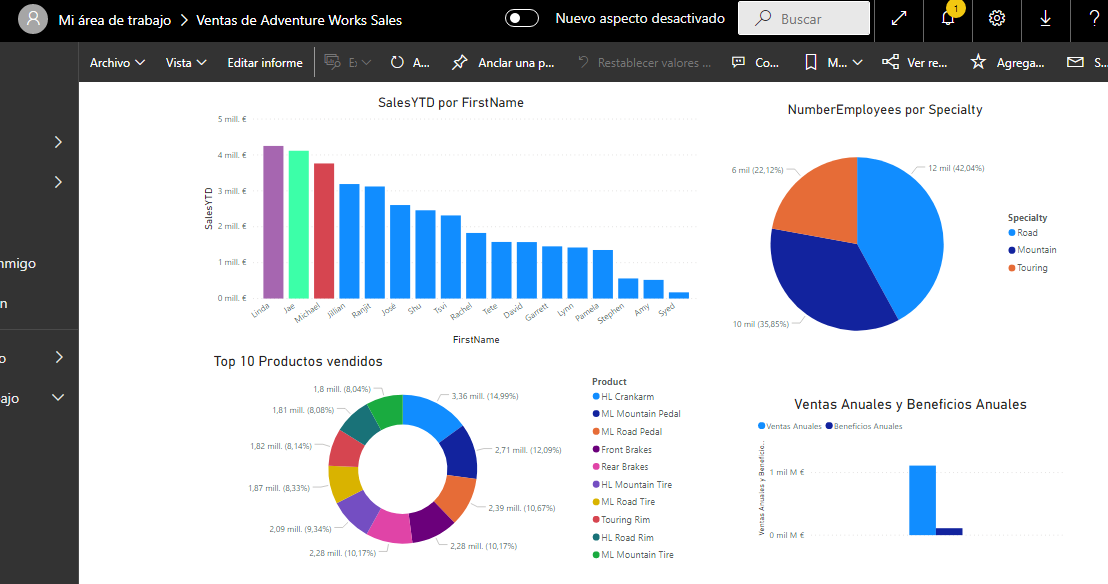
\includegraphics[width=14cm]{./Imagenes/tarea3_1}}
	\end{center}
	\end{figure}

\end{itemize}
		
\section{CONCLUSIONES}
Como podemos apreciar, hoy tenemos una tecnología disponible desde hace unos años que nos permite ir a otro nivel de virtualización distinto, permitiéndonos obtener las siguientes ventajas:
\begin{itemize}
\item Instalación simple y capacidad de ejecutar múltiples aplicaciones en entornos aislados sobre un mismo sistema operativo,  permitiéndonos ahorrar horas de trabajo en la administración de Infraestructura.
\item Independiente a la plataforma, permite contar con soluciones más portables.
\item Despliegue de Aplicaciones mucho más rápida y flexible.
\item Disponible en múltiples proveedores de Nube.
	
\end{itemize}

\newpage


\end{document}
